%!TeX root=../houndtop.tex
\chapter{The Light upon the Moor}

\lettrine[lines=4]{S}{econd} report of Dr Watson. \\
\begin{flushright}
\hfill\begin{minipage}{0.3\linewidth}\textsc{Baskerville Hall\\Oct. 15\textsuperscript{th}.}\end{minipage}
\end{flushright}
%\vspace{5pt}

\textsc{My dear Holmes},—If I was compelled to leave you without much news during the early days of my mission you must acknowledge that I am making up for lost time, and that events are now crowding thick and fast upon us. In my last report I ended upon my top note with Barrymore at the window, and now I have quite a budget already which will, unless I am much mistaken, considerably surprise you. Things have taken a turn which I could not have anticipated. In some ways they have within the last forty-eight hours become much clearer and in some ways they have become more complicated. But I will tell you all and you shall judge for yourself.

Before breakfast on the morning following my adventure I went down the corridor and examined the room in which Barrymore had been on the night before. The western window through which he had stared so intently has, I noticed, one peculiarity above all other windows in the house—it commands the nearest outlook on the moor. There is an opening between two trees which enables one from this point of view to look right down upon it, while from all the other windows it is only a distant glimpse which can be obtained. It follows, therefore, that Barrymore, since only this window would serve the purpose, must have been looking out for something or somebody upon the moor. The night was very dark, so that I can hardly imagine how he could have hoped to see anyone. It had struck me that it was possible that some love intrigue was on foot. That would have accounted for his stealthy movements and also for the uneasiness of his wife. The man is a striking-looking fellow, very well equipped to steal the heart of a country girl, so that this theory seemed to have something to support it. That opening of the door which I had heard after I had returned to my room might mean that he had gone out to keep some clandestine appointment. So I reasoned with myself in the morning, and I tell you the direction of my suspicions, however much the result may have shown that they were unfounded.

But whatever the true explanation of Barrymore's movements might be, I felt that the responsibility of keeping them to myself until I could explain them was more than I could bear. I had an interview with the baronet in his study after breakfast, and I told him all that I had seen. He was less surprised than I had expected.

»I knew that Barrymore walked about nights, and I had a mind to speak to him about it,« said he. »Two or three times I have heard his steps in the passage, coming and going, just about the hour you name.«

»Perhaps then he pays a visit every night to that particular window,« I suggested.

»Perhaps he does. If so, we should be able to shadow him, and see what it is that he is after. I wonder what your friend Holmes would do, if he were here.«

»I believe that he would do exactly what you now suggest,« said I. »He would follow Barrymore and see what he did.«

»Then we shall do it together.«

»But surely he would hear us.«

»The man is rather deaf, and in any case we must take our chance of that. We'll sit up in my room to-night and wait until he passes.« Sir Henry rubbed his hands with pleasure, and it was evident that he hailed the adventure as a relief to his somewhat quiet life upon the moor.

The baronet has been in communication with the architect who prepared the plans for Sir Charles, and with a contractor from London, so that we may expect great changes to begin here soon. There have been decorators and furnishers up from Plymouth, and it is evident that our friend has large ideas, and means to spare no pains or expense to restore the grandeur of his family. When the house is renovated and refurnished, all that he will need will be a wife to make it complete. Between ourselves there are pretty clear signs that this will not be wanting if the lady is willing, for I have seldom seen a man more infatuated with a woman than he is with our beautiful neighbour, Miss Stapleton. And yet the course of true love does not run quite as smoothly as one would under the circumstances expect. To-day, for example, its surface was broken by a very unexpected ripple, which has caused our friend considerable perplexity and annoyance.

After the conversation which I have quoted about Barrymore, Sir Henry put on his hat and prepared to go out. As a matter of course I did the same.

»What, are \emph{you} coming, Watson?« he asked, looking at me in a curious way.

»That depends on whether you are going on the moor,« said I.

»Yes, I am.«

»Well, you know what my instructions are. I am sorry to intrude, but you heard how earnestly Holmes insisted that I should not leave you, and especially that you should not go alone upon the moor.«

Sir Henry put his hand upon my shoulder with a pleasant smile.

»My dear fellow,« said he, »Holmes, with all his wisdom, did not foresee some things which have happened since I have been on the moor. You understand me? I am sure that you are the last man in the world who would wish to be a spoil-sport. I must go out alone.«

It put me in a most awkward position. I was at a loss what to say or what to do, and before I had made up my mind he picked up his cane and was gone.

But when I came to think the matter over my conscience reproached me bitterly for having on any pretext allowed him to go out of my sight. I imagined what my feelings would be if I had to return to you and to confess that some misfortune had occurred through my disregard for your instructions. I assure you my cheeks flushed at the very thought. It might not even now be too late to overtake him, so I set off at once in the direction of Merripit House.

I hurried along the road at the top of my speed without seeing anything of Sir Henry, until I came to the point where the moor path branches off. There, fearing that perhaps I had come in the wrong direction after all, I mounted a hill from which I could command a view—the same hill which is cut into the dark quarry. Thence I saw him at once. He was on the moor path, about a quarter of a mile off, and a lady was by his side who could only be Miss Stapleton. It was clear that there was already an understanding between them and that they had met by appointment. They were walking slowly along in deep conversation, and I saw her making quick little movements of her hands as if she were very earnest in what she was saying, while he listened intently, and once or twice shook his head in strong dissent. I stood among the rocks watching them, very much puzzled as to what I should do next. To follow them and break into their intimate conversation seemed to be an outrage, and yet my clear duty was never for an instant to let him out of my sight. To act the spy upon a friend was a hateful task. Still, I could see no better course than to observe him from the hill, and to clear my conscience by confessing to him afterwards what I had done. It is true that if any sudden danger had threatened him I was too far away to be of use, and yet I am sure that you will agree with me that the position was very difficult, and that there was nothing more which I could do.

\begin{figure}[h!]
\centering

\includegraphics[width=.9\linewidth]{09_drewmiss}
\caption{Sir Henry suddenly drew Miss Stapleton to his side.}
\end{figure}

Our friend, Sir Henry, and the lady had halted on the path and were standing deeply absorbed in their conversation, when I was suddenly aware that I was not the only witness of their interview. A wisp of green floating in the air caught my eye, and another glance showed me that it was carried on a stick by a man who was moving among the broken ground. It was Stapleton with his butterfly-net. He was very much closer to the pair than I was, and he appeared to be moving in their direction. At this instant Sir Henry suddenly drew Miss Stapleton to his side. His arm was round her, but it seemed to me that she was straining away from him with her face averted. He stooped his head to hers, and she raised one hand as if in protest. Next moment I saw them spring apart and turn hurriedly round. Stapleton was the cause of the interruption. He was running wildly towards them, his absurd net dangling behind him. He gesticulated and almost danced with excitement in front of the lovers. What the scene meant I could not imagine, but it seemed to me that Stapleton was abusing Sir Henry, who offered explanations, which became more angry as the other refused to accept them. The lady stood by in haughty silence. Finally Stapleton turned upon his heel and beckoned in a peremptory way to his sister, who, after an irresolute glance at Sir Henry, walked off by the side of her brother. The naturalist's angry gestures showed that the lady was included in his displeasure. The baronet stood for a minute looking after them, and then he walked slowly back the way that he had come, his head hanging, the very picture of dejection.

What all this meant I could not imagine, but I was deeply a\-shamed to have witnessed so intimate a scene without my friend's knowledge. I ran down the hill therefore and met the baronet at the bottom. His face was flushed with anger and his brows were wrin\-kled, like one who is at his wit's ends what to do.

»Halloa, Watson! Where have you dropped from?« said he. »You don't mean to say that you came after me in spite of all?«

I explained everything to him: how I had found it impossible to remain behind, how I had followed him, and how I had witnessed all that had occurred. For an instant his eyes blazed at me, but my frankness disarmed his anger, and he broke at last into a rather rueful laugh.

»You would have thought the middle of that prairie a fairly safe place for a man to be private,« said he, »but, by thunder, the whole country-side seems to have been out to see me do my wooing—and a mighty poor wooing at that! Where had you engaged a seat?«

»I was on that hill.«

»Quite in the back row, eh? But her brother was well up to the front. Did you see him come out on us?«

»Yes, I did.«

»Did he ever strike you as being crazy—this brother of hers?«

»I can't say that he ever did.«

»I dare say not. I always thought him sane enough until to-day, but you can take it from me that either he or I ought to be in a strait-jacket. What's the matter with me, anyhow? You've lived near me for some weeks, Watson. Tell me straight, now! Is there anything that would prevent me from making a good husband to a woman that I loved?«

»I should say not.«

»He can't object to my worldly position, so it must be myself that he has this down on. What has he against me? I never hurt man or woman in my life that I know of. And yet he would not so much as let me touch the tips of her fingers.«

»Did he say so?«

»That, and a deal more. I tell you, Watson, I've only known her these few weeks, but from the first I just felt that she was made for me, and she, too—she was happy when she was with me, and that I'll swear. There's a light in a woman's eyes that speaks louder than words. But he has never let us get together, and it was only to-day for the first time that I saw a chance of having a few words with her alone. She was glad to meet me, but when she did it was not love that she would talk about, and she wouldn't have let me talk about it either if she could have stopped it. She kept coming back to it that this was a place of danger, and that she would never be happy until I had left it. I told her that since I had seen her I was in no hurry to leave it, and that if she really wanted me to go, the only way to work it was for her to arrange to go with me. With that I offered in as many words to marry her, but before she could answer, down came this brother of hers, running at us with a face on him like a madman. He was just white with rage, and those light eyes of his were blazing with fury. What was I doing with the lady? How dared I offer her attentions which were distasteful to her? Did I think that because I was a baronet I could do what I liked? If he had not been her brother I should have known better how to answer him. As it was I told him that my feelings towards his sister were such as I was not ashamed of, and that I hoped that she might honour me by becoming my wife. That seemed to make the matter no better, so then I lost my temper too, and I answered him rather more hotly than I should perhaps, considering that she was standing by. So it ended by his going off with her, as you saw, and here am I as badly puzzled a man as any in this county. Just tell me what it all means, Watson, and I'll owe you more than ever I can hope to pay.«

I tried one or two explanations, but, indeed, I was completely puzzled myself. Our friend's title, his fortune, his age, his character, and his appearance are all in his favour, and I know nothing against him unless it be this dark fate which runs in his family. That his advances should be rejected so brusquely without any reference to the lady's own wishes, and that the lady should accept the situation without protest, is very amazing. However, our conjectures were set at rest by a visit from Stapleton himself that very afternoon. He had come to offer apologies for his rudeness of the morning, and after a long private interview with Sir Henry in his study, the upshot of their conversation was that the breach is quite healed, and that we are to dine at Merripit House next Friday as a sign of it.

»I don't say now that he isn't a crazy man,« said Sir Henry; »I can't forget the look in his eyes when he ran at me this morning, but I must allow that no man could make a more handsome apology than he has done.«

»Did he give any explanation of his conduct?«

»His sister is everything in his life, he says. That is natural e\-nough, and I am glad that he should understand her value. They have always been together, and according to his account he has been a very lonely man with only her as a companion, so that the thought of losing her was really terrible to him. He had not understood, he said, that I was becoming attached to her, but when he saw with his own eyes that it was really so, and that she might be taken away from him, it gave him such a shock that for a time he was not responsible for what he said or did. He was very sorry for all that had passed, and he recognized how foolish and how selfish it was that he should imagine that he could hold a beautiful woman like his sister to himself for her whole life. If she had to leave him he had rather it was to a neighbour like myself than to anyone else. But in any case it was a blow to him, and it would take him some time before he could prepare himself to meet it. He would withdraw all opposition upon his part if I would promise for three months to let the matter rest and to be content with cultivating the lady's friendship during that time without claiming her love. This I promised, and so the matter rests.«

So there is one of our small mysteries cleared up. It is something to have touched bottom anywhere in this bog in which we are floundering. We know now why Stapleton looked with disfavour upon his sister's suitor—even when that suitor was so eligible a one as Sir Henry. And now I pass on to another thread which I have extricated out of the tangled skein, the mystery of the sobs in the night, of the tear-stained face of Mrs Barrymore, of the secret journey of the butler to the western lattice window. Congratulate me, my dear Holmes, and tell me that I have not disappointed you as an agent—that you do not regret the confidence which you showed in me when you sent me down. All these things have by one night's work been thoroughly cleared.

I have said »by one night's work,« but, in truth, it was by two nights' work, for on the first we drew entirely blank. I sat up with Sir Henry in his rooms until nearly three o'clock in the morning, but no sound of any sort did we hear except the chiming clock upon the stairs. It was a most melancholy vigil, and ended by each of us falling asleep in our chairs. Fortunately we were not discouraged, and we determined to try again. The next night we lowered the lamp, and sat smoking cigarettes without making the least sound. It was incredible how slowly the hours crawled by, and yet we were helped through it by the same sort of patient interest which the hunter must feel as he watches the trap into which he hopes the game may wander. One struck, and two, and we had almost for the second time given it up in despair, when in an instant we both sat bolt upright in our chairs, with all our weary senses keenly on the alert once more. We had heard the creak of a step in the passage.

\begin{wrapfigure}{O}{0.7\textwidth}
\centering

\includegraphics[width=.7\linewidth]{09_doinghere}
\caption{»What are you doing here, Barrymore?«}
\end{wrapfigure}

Very stealthily we heard it pass along until it died away in the distance. Then the baronet gently opened his door and we set out in pursuit. Already our man had gone round the gallery, and the corridor was all in darkness. Softly we stole along until we had come into the other wing. We were just in time to catch a glimpse of the tall, black-bearded figure, his shoulders rounded, as he tip-toed down the passage. Then he passed through the same door as before, and the light of the candle framed it in the darkness and shot one single yellow beam across the gloom of the corridor. We shuffled cautiously towards it, trying every plank before we dared to put our whole weight upon it. We had taken the precaution of leaving our boots behind us, but, even so, the old boards snapped and creaked beneath our tread. Sometimes it seemed impossible that he should fail to hear our approach. However, the man is fortunately rather deaf, and he was entirely preoccupied in that which he was doing. When at last we reached the door and peeped through we found him crouching at the window, candle in hand, his white, intent face pressed against the pane, exactly as I had seen him two nights before.

We had arranged no plan of campaign, but the baronet is a man to whom the most direct way is always the most natural. He walked into the room, and as he did so Barrymore sprang up from the window with a sharp hiss of his breath and stood, livid and trembling, before us. His dark eyes, glaring out of the white mask of his face, were full of horror and astonishment as he gazed from Sir Henry to me.

»What are you doing here, Barrymore?«

»Nothing, sir.« His agitation was so great that he could hardly speak, and the shadows sprang up and down from the shaking of his candle. »It was the window, sir. I go round at night to see that they are fastened.«

»On the second floor?«

»Yes, sir, all the windows.«

»Look here, Barrymore,« said Sir Henry, sternly; »we have made up our minds to have the truth out of you, so it will save you trouble to tell it sooner rather than later. Come, now! No lies! What were you doing at that window?«

The fellow looked at us in a helpless way, and he wrung his hands together like one who is in the last extremity of doubt and misery.

»I was doing no harm, sir. I was holding a candle to the window.«

»And why were you holding a candle to the window?«

»Don't ask me, Sir Henry—don't ask me! I give you my word, sir, that it is not my secret, and that I cannot tell it. If it concerned no one but myself I would not try to keep it from you.«

A sudden idea occurred to me, and I took the candle from the trembling hand of the butler.

»He must have been holding it as a signal,« said I. »Let us see if there is any answer.« I held it as he had done, and stared out into the darkness of the night. Vaguely I could discern the black bank of the trees and the lighter expanse of the moor, for the moon was behind the clouds. And then I gave a cry of exultation, for a tiny pin-point of yellow light had suddenly transfixed the dark veil, and glowed steadily in the centre of the black square framed by the window.

»There it is!« I cried.

»No, no, sir, it is nothing—nothing at all!« the butler broke in; »I assure you, sir\longdash«

»Move your light across the window, Watson!« cried the baronet. »See, the other moves also! Now, you rascal, do you deny that it is a signal? Come, speak up! Who is your confederate out yonder, and what is this conspiracy that is going on?«

The man's face became openly defiant.

»It is my business, and not yours. I will not tell.«

»Then you leave my employment right away.«

»Very good, sir. If I must I must.«

»And you go in disgrace. By thunder, you may well be ashamed of yourself. Your family has lived with mine for over a hundred years under this roof, and here I find you deep in some dark plot against me.«

»No, no, sir; no, not against you!« It was a woman's voice, and Mrs Barrymore, paler and more horror-struck than her husband, was standing at the door. Her bulky figure in a shawl and skirt might have been comic were it not for the intensity of feeling upon her face.

»We have to go, Eliza. This is the end of it. You can pack our things,« said the butler.

»Oh, John, John, have I brought you to this? It is my doing, Sir Henry—all mine. He has done nothing except for my sake and because I asked him.«

»Speak out, then! What does it mean?«

»My unhappy brother is starving on the moor. We cannot let him perish at our very gates. The light is a signal to him that food is ready for him, and his light out yonder is to show the spot to which to bring it.«

»Then your brother is\longdash«

»The escaped convict, sir—Selden, the criminal.«

»That's the truth, sir,« said Barrymore. »I said that it was not my secret and that I could not tell it to you. But now you have heard it, and you will see that if there was a plot it was not against you.«

\begin{figure}[h!]
\centering
\includegraphics[width=\linewidth]{09_escaped}
\caption{»The escaped convict, sir—Selden, the criminal.«}
\end{figure}

This, then, was the explanation of the stealthy expeditions at night and the light at the window. Sir Henry and I both stared at the woman in amazement. Was it possible that this stolidly respectable person was of the same blood as one of the most notorious criminals in the country?

»Yes, sir, my name was Selden, and he is my younger brother. We humoured him too much when he was a lad, and gave him his own way in everything until he came to think that the world was made for his pleasure, and that he could do what he liked in it. Then as he grew older he met wicked companions, and the devil entered into him until he broke my mother's heart and dragged our name in the dirt. From crime to crime he sank lower and lower, until it is only the mercy of God which has snatched him from the scaffold; but to me, sir, he was always the little curly-headed boy that I had nursed and played with, as an elder sister would. That was why he broke prison, sir. He knew that I was here and that we could not refuse to help him. When he dragged himself here one night, weary and starving, with the warders hard at his heels, what could we do? We took him in and fed him and cared for him. Then you returned, sir, and my brother thought he would be safer on the moor than anywhere else until the hue and cry was over, so he lay in hiding there. But every second night we made sure if he was still there by putting a light in the window, and if there was an answer my husband took out some bread and meat to him. Every day we hoped that he was gone, but as long as he was there we could not desert him. That is the whole truth, as I am an honest Christian woman, and you will see that if there is blame in the matter it does not lie with my husband, but with me, for whose sake he has done all that he has.«

The woman's words came with an intense earnestness which carried conviction with them.

»Is this true, Barrymore?«

»Yes, Sir Henry. Every word of it.«

»Well, I cannot blame you for standing by your own wife. Forget what I have said. Go to your room, you two, and we shall talk further about this matter in the morning.«

When they were gone we looked out of the window again. Sir Henry had flung it open, and the cold night wind beat in upon our faces. Far away in the black distance there still glowed that one tiny point of yellow light.

»I wonder he dares,« said Sir Henry.

»It may be so placed as to be only visible from here.«

»Very likely. How far do you think it is?«

»Out by the Cleft Tor, I think.«

»Not more than a mile or two off.«

»Hardly that.«

»Well, it cannot be far if Barrymore had to carry out the food to it. And he is waiting, this villain, beside that candle. By thunder, Watson, I am going out to take that man!«

The same thought had crossed my own mind. It was not as if the Barrymores had taken us into their confidence. Their secret had been forced from them. The man was a danger to the community, an unmitigated scoundrel for whom there was neither pity nor excuse. We were only doing our duty in taking this chance of putting him back where he could do no harm. With his brutal and violent nature, others would have to pay the price if we held our hands. Any night, for example, our neighbours the Stapletons might be attacked by him, and it may have been the thought of this which made Sir Henry so keen upon the adventure.

»I will come,« said I.

»Then get your revolver and put on your boots. The sooner we start the better, as the fellow may put out his light and be off.«

In five minutes we were outside the door, starting upon our expedition. We hurried through the dark shrubbery, amid the dull moaning of the autumn wind and the rustle of the falling leaves. The night air was heavy with the smell of damp and decay. Now and again the moon peeped out for an instant, but clouds were driving over the face of the sky, and just as we came out on the moor a thin rain began to fall. The light still burned steadily in front.

»Are you armed?« I asked.

»I have a hunting-crop.«

»We must close in on him rapidly, for he is said to be a desperate fellow. We shall take him by surprise and have him at our mercy before he can resist.«

»I say, Watson,« said the baronet, »what would Holmes say to this? How about that hour of darkness in which the power of evil is exalted?«

As if in answer to his words there rose suddenly out of the vast gloom of the moor that strange cry which I had already heard upon the borders of the great Grimpen Mire. It came with the wind through the silence of the night, a long, deep mutter, then a rising howl, and then the sad moan in which it died away. Again and again it sounded, the whole air throbbing with it, strident, wild, and menacing. The baronet caught my sleeve and his face glimmered white through the darkness.



»My God, what's that, Watson?«

»I don't know. It's a sound they have on the moor. I heard it once before.«

It died away, and an absolute silence closed in upon us. We stood straining our ears, but nothing came.

»Watson,« said the baronet, »it was the cry of a hound.«

My blood ran cold in my veins, for there was a break in his voice which told of the sudden horror which had seized him.

»What do they call this sound?« he asked.

»Who?«

\makeatletter
\@ifclasswith{scrbook}{a5paper}
{%
%	\begin{figure}[h!]
%	\centering
\begin{center}
	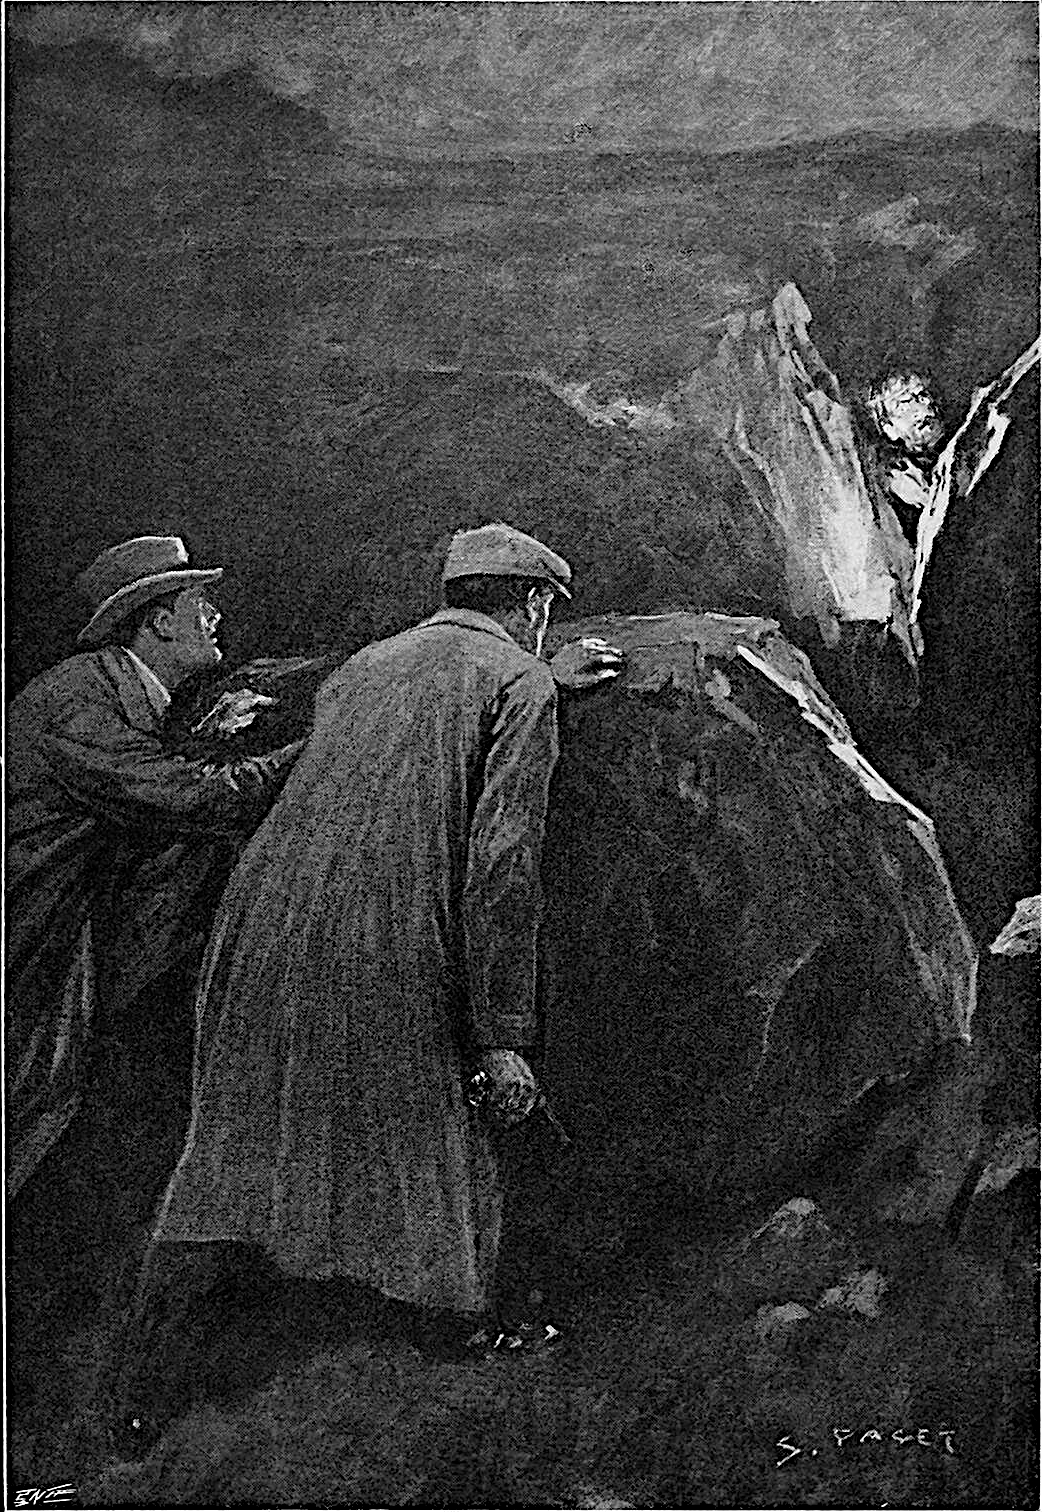
\includegraphics[width=.95\linewidth]{09_evilface}
	%\caption{Over the rocks was thrust out an evil yellow face}
	\captionof{figure}{Over the rocks was thrust out an evil yellow face}
\end{center}
\thispagestyle{empty}
\clearpage
%	\end{figure}
}{%

}

\makeatother


\makeatletter
\@ifclasswith{scrbook}{a5paper}
{%

}{%
	\begin{figure}[h!]
	\centering
	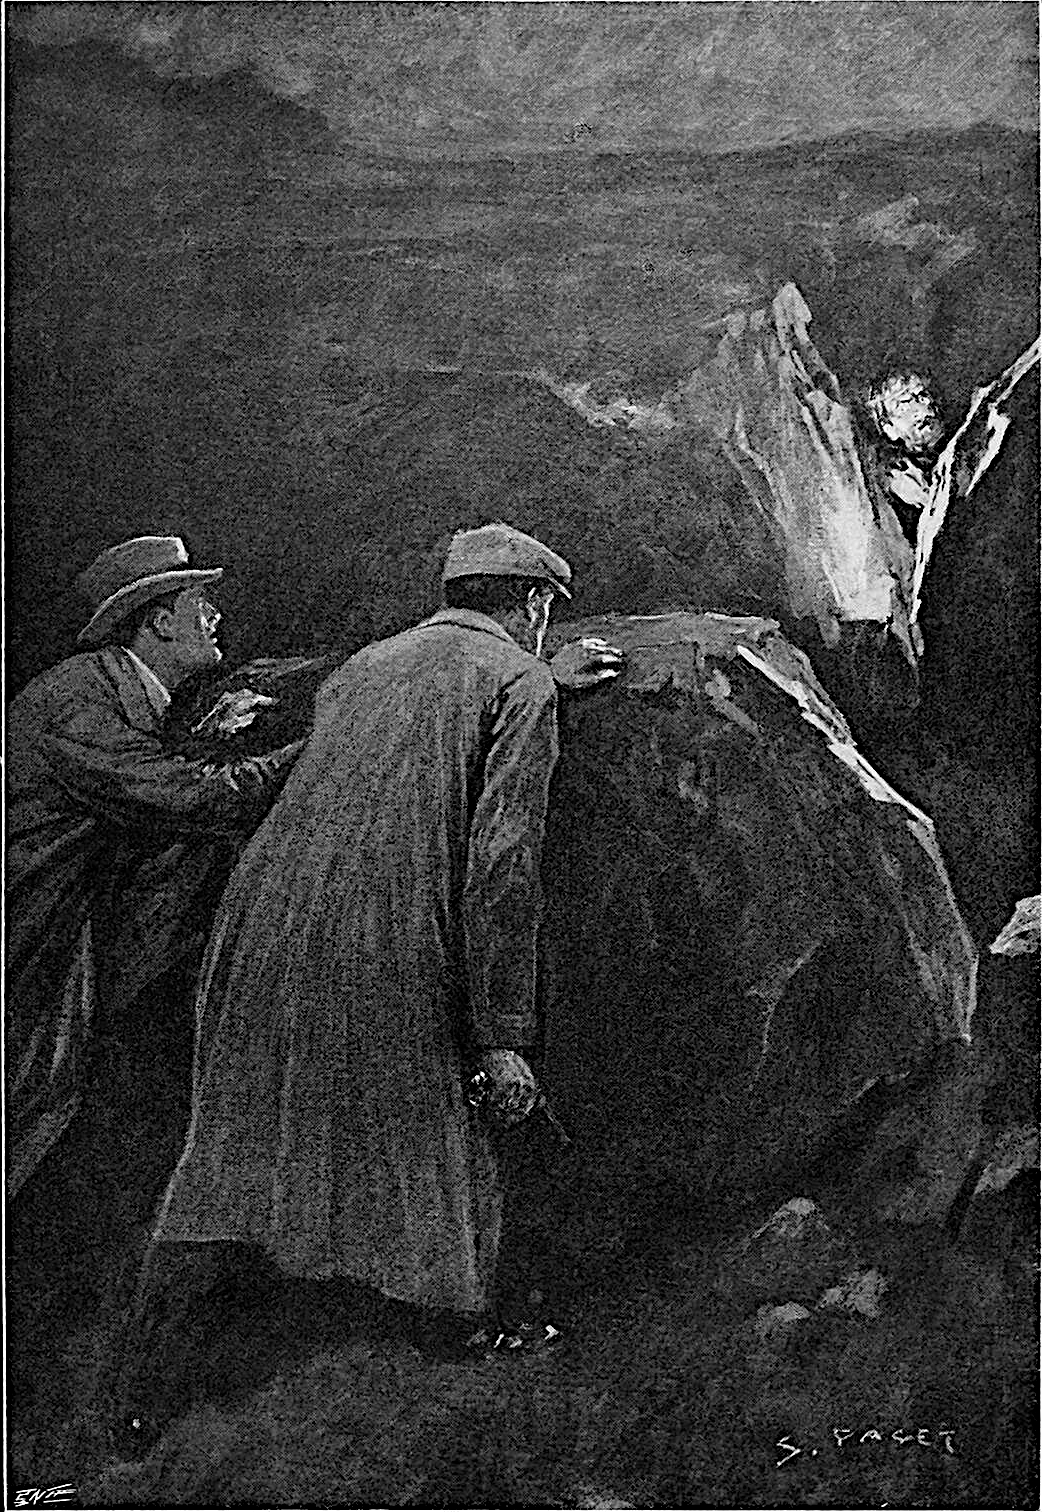
\includegraphics[width=\linewidth]{09_evilface}
	\caption{Over the rocks was thrust out an evil yellow face}
	\end{figure}
}

\makeatother

»The folk on the country-side.«

»Oh, they are ignorant people. Why should you mind what they call it?«

 
»Tell me, Watson. What do they say of it?«

I hesitated but could not escape the question.

»They say it is the cry of the Hound of the Baskervilles.«

He groaned and was silent for a few moments.

»A hound it was,« he said, at last, »but it seemed to come from miles away, over yonder, I think.«

»It was hard to say whence it came.«

»It rose and fell with the wind. Isn't that the direction of the great Grimpen Mire?«

»Yes, it is.«

»Well, it was up there. Come now, Watson, didn't you think yourself that it was the cry of a hound? I am not a child. You need not fear to speak the truth.«

»Stapleton was with me when I heard it last. He said that it might be the calling of a strange bird.«

»No, no, it was a hound. My God, can there be some truth in all these stories? Is it possible that I am really in danger from so dark a cause? You don't believe it, do you, Watson?«

»No, no.«

»And yet it was one thing to laugh about it in London, and it is another to stand out here in the darkness of the moor and to hear such a cry as that. And my uncle! There was the footprint of the hound beside him as he lay. It all fits together. I don't think that I am a coward, Watson, but that sound seemed to freeze my very blood. Feel my hand!«

It was as cold as a block of marble.

»You'll be all right to-morrow.«

»I don't think I'll get that cry out of my head. What do you advise that we do now?«

»Shall we turn back?«

»No, by thunder; we have come out to get our man, and we will do it. We after the convict, and a hell-hound, as likely as not, after us. Come on! We'll see it through if all the fiends of the pit were loose upon the moor.«

We stumbled slowly along in the darkness, with the black loom of the craggy hills around us, and the yellow speck of light burning steadily in front. There is nothing so deceptive as the distance of a light upon a pitch-dark night, and sometimes the glimmer seemed to be far away upon the horizon and sometimes it might have been within a few yards of us. But at last we could see whence it came, and then we knew that we were indeed very close. A guttering candle was stuck in a crevice of the rocks which flanked it on each side so as to keep the wind from it and also to prevent it from being visible, save in the direction of Baskerville Hall. A boulder of granite concealed our approach, and crouching behind it we gazed over it at the signal light. It was strange to see this single candle burning there in the middle of the moor, with no sign of life near it—just the one straight yellow flame and the gleam of the rock on each side of it.



»What shall we do now?« whispered Sir Henry.

»Wait here. He must be near his light. Let us see if we can get a glimpse of him.«

The words were hardly out of my mouth when we both saw him. Over the rocks, in the crevice of which the candle burned, there was thrust out an evil yellow face, a terrible animal face, all seamed and scored with vile passions. Foul with mire, with a bristling beard, and hung with matted hair, it might well have belonged to one of those old savages who dwelt in the burrows on the hillsides. The light beneath him was reflected in his small, cunning eyes which peered fiercely to right and left through the darkness, like a crafty and savage animal who has heard the steps of the hunters.

Something had evidently aroused his suspicions. It may have been that Barrymore had some private signal which we had neglected to give, or the fellow may have had some other reason for thinking that all was not well, but I could read his fears upon his wicked face. Any instant he might dash out the light and vanish in the darkness. I sprang forward therefore, and Sir Henry did the same. At the same moment the convict screamed out a curse at us and hurled a rock which splintered up against the boulder which had sheltered us. I caught one glimpse of his short, squat, strongly- built figure as he sprang to his feet and turned to run. At the same moment by a lucky chance the moon broke through the clouds. We rushed over the brow of the hill, and there was our man running with great speed down the other side, springing over the stones in his way with the activity of a mountain goat. A lucky long shot of my revolver might have crippled him, but I had brought it only to defend myself if attacked, and not to shoot an unarmed man who was running away.


We were both swift runners and in fairly good training, but we soon found that we had no chance of overtaking him. We saw him for a long time in the moonlight until he was only a small speck moving swiftly among the boulders upon the side of a distant hill. We ran and ran until we were completely blown, but the space between us grew ever wider. Finally we stopped and sat panting on two rocks, while we watched him disappearing in the distance.

\makeatletter
\@ifclasswith{scrbook}{a5paper}
{%
	\begin{figure}[p]
	\centering
	
\includegraphics[width=\linewidth]{09_manontor}
	\caption{I saw the figure of a man upon the tor}
	\end{figure}
}{%

}

\makeatother

And it was at this moment that there occurred a most strange and unexpected thing. We had risen from our rocks and were turning to go home, having abandoned the hopeless chase. The moon was low upon the right, and the jagged pinnacle of a granite tor stood up against the lower curve of its silver disc. There, outlined as black as an ebony statue on that shining back-ground, I saw the figure of a man upon the tor. Do not think that it was a delusion, Holmes. I assure you that I have never in my life seen anything more clearly. As far as I could judge, the figure was that of a tall, thin man. He stood with his legs a little separated, his arms folded, his head bowed, as if he were brooding over that enormous wilderness of peat and granite which lay before him. He might have been the very spirit of that terrible place. It was not the convict. This man was far from the place where the latter had disappeared. Besides, he was a much taller man. With a cry of surprise I pointed him out to the baronet, but in the instant during which I had turned to grasp his arm the man was gone. There was the sharp pinnacle of granite still cutting the lower edge of the moon, but its peak bore no trace of that silent and motionless figure.

\makeatletter
\@ifclasswith{scrbook}{a5paper}
{%

}{%
	\begin{figure}[p]
	\centering
	
\includegraphics[width=\linewidth]{09_manontor}
	\caption{I saw the figure of a man upon the tor}
	\end{figure}
}

\makeatother



I wished to go in that direction and to search the tor, but it was some distance away. The baronet's nerves were still quivering from that cry, which recalled the dark story of his family, and he was not in the mood for fresh adventures. He had not seen this lonely man upon the tor and could not feel the thrill which his strange presence and his commanding attitude had given to me. »A warder, no doubt,« said he. »The moor has been thick with them since this fellow escaped.« Well, perhaps his explanation may be the right one, but I should like to have some further proof of it. To-day we mean to communicate to the Princetown people where they should look for their missing man, but it is hard lines that we have not actually had the triumph of bringing him back as our own prisoner. Such are the adventures of last night, and you must acknowledge, my dear Holmes, that I have done you very well in the matter of a report. Much of what I tell you is no doubt quite irrelevant, but still I feel that it is best that I should let you have all the facts and leave you to select for yourself those which will be of most service to you in helping you to your conclusions. We are certainly making some progress. So far as the Barrymores go we have found the motive of their actions, and that has cleared up the situation very much. But the moor with its mysteries and its strange inhabitants remains as inscrutable as ever. Perhaps in my next I may be able to throw some light upon this also. Best of all would it be if you could come down to us. In any case you will hear from me again in the course of the next few days.

%\cleardoubleevenpage
%\vfill
%\begin{figure}[tbph]
%\centering
%\includegraphics[width=1\linewidth]{craggy}
%\caption{From its craggy summit I looked out myself across the melancholy downs.}
%\end{figure}
%\vfill
%\thispagestyle{empty}
%\clearpage
